\documentclass[11pt]{article}

\usepackage{sectsty}
\usepackage{graphicx}
\usepackage{float}

% Margins
\topmargin=-0.45in
\evensidemargin=0in
\oddsidemargin=0in
\textwidth=6.5in
\textheight=9.0in
\headsep=0.25in

\title{CS 3600 Lab Project Phase 1}
\author{Jake Gendreau, Michael Crapse}
\date{\today}

\begin{document}
\maketitle	

\tableofcontents
\newpage

\section{Project Plan}
    The goal of this project is to create an inventory management system for the Vandal Marching Band. It should be able to keep track
    of students, what clothing pieces they have rented, and what instrument(s) they have rented. The core features are as follows
    \begin{itemize}
        \item Add / remove students from the system.
        \item Add / remove clothing items from the system.
        \item Add / remove instruments from the system.
        \item Associate a student with any number of clothing pieces and any number of instruments.
        \item Be able to search the database for students, clothing pieces, and instruments.
    \end{itemize}

\section{Technology Stack}
    \subsection{Backend}
        \subsubsection{Language} For our backend language, we will be utilizing Python. We chose python for a few reasons:
        \begin{enumerate}
            \item \textbf{Documentation and Support:} Python is an extremely well documented and supported language, and as a result, many StackOverflow
            forms, Reddit threads, or the actual documentation will have everything that we need to solve any problems we
            may face.
            \item \textbf{Libraries:} Extremely well supported libraries make implementing the features that we want to
            a much easier task than it would be if we had to implement them from scratch. Libraries such as Django
            or Flask for the web server provide extremely refined and well documented solutions for the features that we wish to add.
        \end{enumerate}

        \subsubsection{Libraries} We will be using several libraries in our project. Primarily, we will be
        using the following:
        \begin{enumerate}
            \item \textbf{Django:} We chose to use Django as our web server because of its "batteries included" approach,
            which means that many features that a website may want to use (e.g. login security, cookies,
            databases) have first-party developed modules which are well documented and easy to add.
        \end{enumerate}

    \subsection{Database}
        Due to our choice to use Python and Django, we were left with a few natively supported options for
        our database management software. After some conversation, we decided that SQLite3 would be the best
        option, as both of us have experience in the software, and the limited installation size and feature 
        set means that it is easier to install, use, and develop with.

\section{Division of Labor}
    Michael and I will be splitting the work evenly down the middle. We have not figured out what exactly each of us will do yet, but
    we will take efforts to ensure that our efforts are equal.

\section{ER Diagram}
    \begin{figure}[H]
        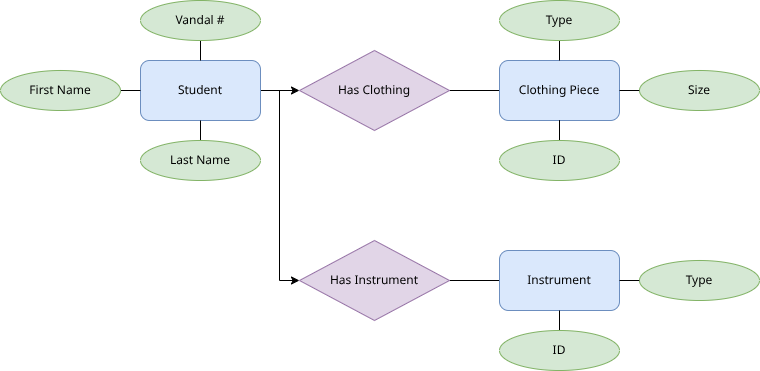
\includegraphics[width=\linewidth]{./ER_Diagram.png}
        \caption{ER Model for VMB Inventory System}
        \label{fig:er_model}
    \end{figure}

\section{Timeline of Deliverables}
    \begin{itemize}
        \item \textbf{March 23, 2026:} The initial draft for the project must be ready, along with
        a presentation about the project.
        \item \textbf{April 15, 2026:} The project must have a finalized database design, all interfaces
        designed, all functions planned out, and at least one functional interface with backend.
        \item \textbf{May 1, 2026:} The project should be fully functional at this point and all aspects of the project should 
        properly interact with minimal bugs
        \item \textbf{May 15, 2026:} The project must be complete by this point.
    \end{itemize}


\end{document}
